% This file was created with tikzplotlib v0.10.1.
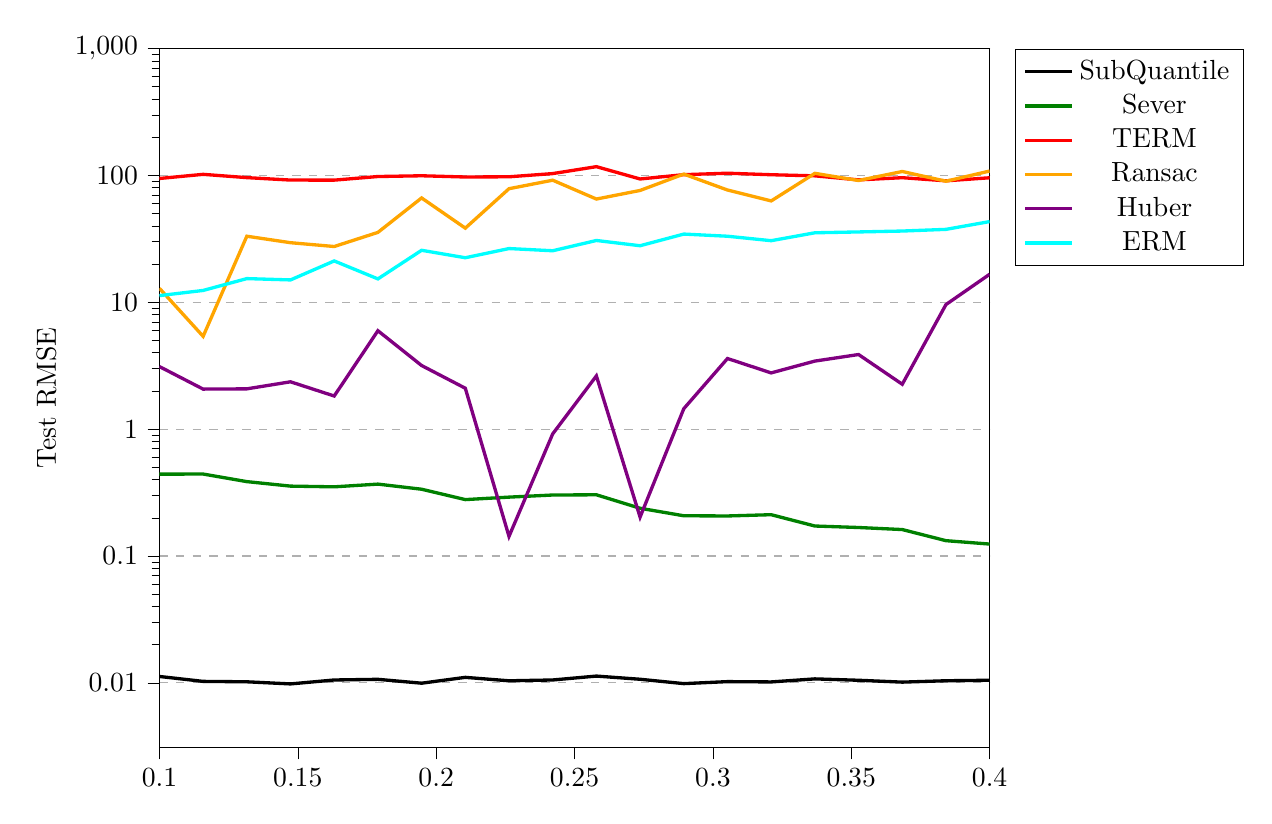
\begin{tikzpicture}

\definecolor{cyan}{RGB}{0,255,255}
\definecolor{darkgray176}{RGB}{176,176,176}
\definecolor{green}{RGB}{0,128,0}
\definecolor{orange}{RGB}{255,165,0}
\definecolor{purple}{RGB}{128,0,128}

\begin{axis}[
tick align=outside,
tick pos=left,
legend pos=outer north east,
x grid style={darkgray176},
xmin=0.1, xmax=0.4,
xtick style={color=black},
y grid style={darkgray176},
ymin=0, ymax=1000,
ytick style={color=black},
ytick={0,0.01,0.1,1,10,100,1000},
ymajorgrids=true,
grid style=dashed,
ymode=log,
log ticks with fixed point,
ylabel=Test RMSE,
width=\textwidth,
]
\addplot [very thick, black]
table {%
0.1 0.0112324198707938
0.115789473684211 0.0102729490026832
0.131578947368421 0.0101964855566621
0.147368421052632 0.00981182046234608
0.163157894736842 0.0105369370430708
0.178947368421053 0.0106649044901133
0.194736842105263 0.00994088780134916
0.210526315789474 0.0110519528388977
0.226315789473684 0.010382934473455
0.242105263157895 0.0105386478826404
0.257894736842105 0.0113116847351193
0.273684210526316 0.0106768608093262
0.289473684210526 0.00986308325082064
0.305263157894737 0.0102291321381927
0.321052631578947 0.0101717608049512
0.336842105263158 0.0107493065297604
0.352631578947369 0.0104831522330642
0.368421052631579 0.010135336779058
0.38421052631579 0.0103916563093662
0.4 0.0104853436350822
};
\addplot [very thick, green]
table {%
0.1 0.441622585058212
0.115789473684211 0.442577987909317
0.131578947368421 0.385704278945923
0.147368421052632 0.355443328619003
0.163157894736842 0.350905865430832
0.178947368421053 0.368659645318985
0.194736842105263 0.335970044136047
0.210526315789474 0.278307229280472
0.226315789473684 0.291088610887527
0.242105263157895 0.302447915077209
0.257894736842105 0.303686618804932
0.273684210526316 0.237833008170128
0.289473684210526 0.207529976963997
0.305263157894737 0.206792339682579
0.321052631578947 0.211597204208374
0.336842105263158 0.172316461801529
0.352631578947369 0.167733907699585
0.368421052631579 0.161582171916962
0.38421052631579 0.132057636976242
0.4 0.124149031937122
};
\addplot [very thick, red]
table {%
0.1 94.5182800292969
0.115789473684211 101.906234741211
0.131578947368421 95.9897155761719
0.147368421052632 91.8465347290039
0.163157894736842 91.7415313720703
0.178947368421053 97.9414749145508
0.194736842105263 99.2902450561523
0.210526315789474 97.1035461425781
0.226315789473684 97.4736709594727
0.242105263157895 103.306343078613
0.257894736842105 117.140129089355
0.273684210526316 93.6604385375977
0.289473684210526 101.311218261719
0.305263157894737 104.010284423828
0.321052631578947 101.181632995605
0.336842105263158 99.1554718017578
0.352631578947369 92.1359710693359
0.368421052631579 95.8898544311523
0.38421052631579 90.5693130493164
0.4 95.7592468261719
};
\addplot [very thick, orange]
table {%
0.1 12.8784780502319
0.115789473684211 5.38716888427734
0.131578947368421 33.1459999084473
0.147368421052632 29.4698734283447
0.163157894736842 27.500358581543
0.178947368421053 35.5395240783691
0.194736842105263 66.3939056396484
0.210526315789474 38.3871383666992
0.226315789473684 78.5180969238281
0.242105263157895 91.6210708618164
0.257894736842105 65.0814895629883
0.273684210526316 76.0701293945312
0.289473684210526 102.360397338867
0.305263157894737 76.6779403686523
0.321052631578947 62.8883666992188
0.336842105263158 103.778694152832
0.352631578947369 91.1223373413086
0.368421052631579 107.335075378418
0.38421052631579 89.9517517089844
0.4 108.187255859375
};
\addplot [very thick, purple]
table {%
0.1 3.11222171783447
0.115789473684211 2.06761121749878
0.131578947368421 2.0770800113678
0.147368421052632 2.36055493354797
0.163157894736842 1.823979139328
0.178947368421053 5.96385192871094
0.194736842105263 3.17209100723267
0.210526315789474 2.10031628608704
0.226315789473684 0.142739579081535
0.242105263157895 0.917115569114685
0.257894736842105 2.62751007080078
0.273684210526316 0.202511191368103
0.289473684210526 1.44876229763031
0.305263157894737 3.60196709632874
0.321052631578947 2.77458095550537
0.336842105263158 3.43842387199402
0.352631578947369 3.87289190292358
0.368421052631579 2.25752830505371
0.38421052631579 9.59063625335693
0.4 16.624475479126
};
\addplot [very thick, cyan]
table {%
0.1 11.2793025970459
0.115789473684211 12.3885202407837
0.131578947368421 15.359691619873
0.147368421052632 14.9969387054443
0.163157894736842 21.1634616851807
0.178947368421053 15.2750644683838
0.194736842105263 25.6762809753418
0.210526315789474 22.4262428283691
0.226315789473684 26.4983062744141
0.242105263157895 25.4622230529785
0.257894736842105 30.6805667877197
0.273684210526316 27.8887958526611
0.289473684210526 34.4648094177246
0.305263157894737 33.139274597168
0.321052631578947 30.5629692077637
0.336842105263158 35.2868499755859
0.352631578947369 35.8248291015625
0.368421052631579 36.4146728515625
0.38421052631579 37.5435447692871
0.4 43.227710723877
};
\legend{SubQuantile,Sever,TERM,Ransac,Huber,ERM}
\end{axis}

\end{tikzpicture}
